SteelEagle, at its core, is born from the insight that commercial-off-the-shelf (COTS) photography drones present the best combination of light weight, low cost, accessibility, and programmability on the market. The majority of these drones are also close to or below international weight regulatory limits, permitting them to fly in populated environments without significant legal hurdles. I maintain that enabling full autonomy on such drones presents the best chance for widespread adoption of fully-autonomous drones in dense urban settings.

The first step in achieving this vision is providing real-time compute resources for these drones via edge computing. This is what enables full autonomy; sensor processing algorithms running at the edge give the drone an understanding of its surroundings, allowing it to make unsupervised decisions on how to proceed. In this chapter I will explain how to establish this connection between drones and the edge using only COTS components. In Sections~\ref{sec:achieving-cell-conn}-\ref{sec:quest-working-stream}, I will discuss the many failed prototypes I tested before arriving at an initial solution.

\section{Design Goals}
Establishing a connection to the edge on any current COTS drone hardware is non-trivial. Doing so on a COTS photography drone is near impossible out-of-the-box. This is the case for the following reasons:
\begin{itemize}
    \item Photography drones are tightly-integrated, black boxes with no ability to change onboard software or hardware. This is because they are meant to be used by novice pilots and so they simplify the user experience at the cost of customizability.
    \item Photography drones usually require a constant connection to the pilot via a controller. This not only mandates a human-in-the-loop but also prevents BVLOS operation.
    \item Photography drones are not designed to carry much payload beyond their stock hardware. They provide no means to power any payload either since their batteries are closed off during flight.
\end{itemize}
These are challenges that any prototype must overcome, regardless of underlying drone platform.
\newpage
For SteelEagle, drones connect to the edge over public 4G/5G cellular. Cellular has excellent coverage in populated areas and has favorable penetration characteristics~\cite{FCC}. This ensures good service wherever SteelEagle drones fly, especially in urban or suburban settings. Unfortunately, at the time of writing this dissertation, no lightweight COTS photography drones are equipped with cellular connectivity; they are designed to be operated within visual line-of-sight of a pilot, a task for which WiFi or RC is well-suited. For my prototype to work, I will have to bring cellular connectivity to a COTS drone without modifying its internal components.

\subsection{Hardware}
For my initial prototype, I chose to work with the Parrot Anafi~\cite{ParrotAnafi}. The Anafi is a COTS photography drone that weighs 320~g and costs \$470. It is equipped with an autopilot that can follow GPS waypoints and perform automatic stabilization. This stabilization involves increasing thrust of rotors to compensate for wind, allowing the drone to maintain its position even in windy conditions. Table~\ref{tab:anafi-features} shows a more detailed specification of the aircraft.

\begin{figure}
    \centering
    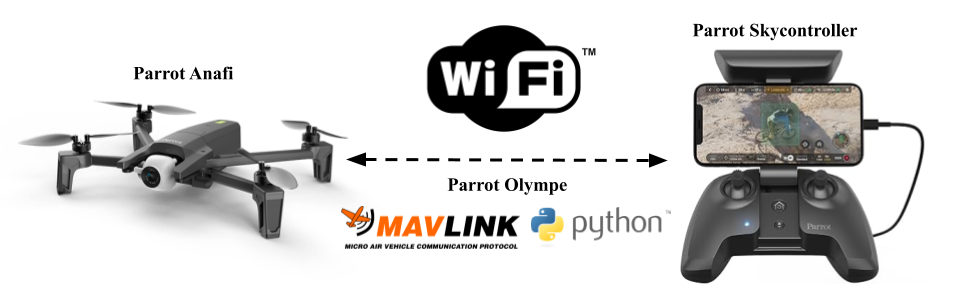
\includegraphics[width=1.0\linewidth]{chapter3/FIGS/ctrl.png}
    \caption{Parrot Remote Control Setup~\cite{ParrotAnafi}}
    \label{fig:parrot-control-setup}
\end{figure}

\begin{table}[]
    \centering
    \rowcolors{2}{gray!10}{white}
    \begin{tabular}{|c|c|}
     \hline
     \textbf{Feature} & \textbf{Description}  \\
     \hline
     Weight & 320~g \\
     \hline
     Cost & \$470 \\
     \hline
     Flight Time & Up to 25 min, in reality 20 min \\
     \hline
     Camera & 4K photo/video \\
     \hline
     Video Stream & 720p 30fps \\
     \hline
     Autopilot* & Custom \\
     \hline
     API & Parrot Olympe / GroundSDK \\
     \hline
     Connectivity & WiFi \\
     \hline
    \end{tabular}
    \begin{captext}
    \\[0.1cm] \small * Drone autopilots manage the low-level control systems onboard, e.g. the ESCs. They usually have the ability to follow GPS waypoints and auto-stabilize under windy conditions. Popular autopilots are ArduPilot and PX4~\cite{Ardupilot,PX4}.
    \end{captext}
    \caption{Parrot Anafi Specifications}
    \label{tab:anafi-features}
\end{table}

\subsubsection{Control Scheme}
The Anafi is designed to be controlled by a human pilot using a remote controller with an attached mobile phone (the Parrot Skycontroller) or exclusively using a mobile phone over WiFi. Alternatively, the drone can also be controlled over WiFi with a Python API called Parrot Olympe or an Android API called Parrot GroundSDK. They are based on the ubiquitous MAVLink protocol~\cite{MAVLink}. Both these APIs grant users high-level flight control and access to telemetry.

Olympe and GroundSDK support two main command types: manual and guided. Manual commands directly actuate the drone. For instance, moving the left stick upwards on the controller would send a manual command to ``increase vertical throttle''. Guided commands, on the other hand, provide the drone with a target to actuate towards. For example, a ``move to this GPS location'' message is a guided command since the drone controls its own actuation towards the specified target.

\subsubsection{Networking}
The drone hosts a WiFi network which supports up to two attached clients. A controller must connect to the WiFi network in order to talk to the drone. This channel may be configured to be either 2.4~GHz or 5~GHz. As reported by Parrot, the connection range of the WiFi channel is around 4~km~\cite{ParrotAnafi}. From my testing, this can fall to around 0.5~km in areas with high wireless interference.

\subsubsection{Video Stream}
A 720p 30fps video stream is generated by the drone and transmitted on its WiFi network via the real-time streaming protocol (RTSP)~\cite{RTSP}. The settings of this stream are not configurable. It is encoded using an intra-refresh slice-decode scheme which is designed to be resilient to packet loss~\cite{Cloudinary}. I will cover the drone's video stream in more detail in Section~\ref{sec:anatomy-drone-stream}.

\subsubsection{Magnetometer}
Most drones are equipped with a magnetometer for discerning bearing. The Parrot Anafi is no exception, though it has an unusually sensitive magnetometer. If the drone's magnetometer detects sufficient interference (e.g. caused by nearby ferromagnetic material~\cite{Ardupilot}), it refuses to fly any guided commands and cancels any guided actuation. This is for safety; if the drone does not have an accurate understanding of its bearing, it may not actuate correctly towards its target and therefore increase the probability of a crash.

\section{Achieving Cellular Connectivity}
\label{sec:achieving-cell-conn}
The Parrot Anafi, like most photography drones, only supports WiFi connectivity and mandates a constant connection to the pilot controller. As stated earlier, the goal of SteelEagle is to use this drone without modification and with an entirely COTS payload.  Thus, any prototype must operate within these constraints. In order to integrate a cellular connection into the loop, it must ensure that from the drone's perspective, it is always connected to what it thinks is a human pilot. One possibility is to mount a router-like device onboard which connects to the drone WiFi and also maintains a cellular connection to the edge. Such a device would have to be light enough to fly but also would need to be able to power itself for the duration of a flight. Ideally, it would also have some internal compute so it can still control the drone during brief network outages.

\subsection{Mobile Phone}
In the COTS mobile device space, one of the best SWaP (size, weight, and power) optimized devices is the mobile phone. Mobile phones have grown immensely powerful in recent years, with some rivaling the power of laptop computers. Furthermore, they are lightweight (usually under 200~g), have a full-featured software development environment, and can power themselves for several hours, even under load. Their connectivity over WiFi and cellular is highly reliable and extensively tested.

In the context of the Parrot Anafi, an Android phone would work well for this purpose, since the Anafi supports an Android API, Parrot GroundSDK. This motivates the following model: an Android phone flies onboard the Parrot Anafi, acting as both a router and a stand-in for the remote controller. By running GroundSDK, the phone will work within the Parrot ecosystem and will therefore maintain the pilot connection that the drone necessitates (Figure~\ref{fig:phone-control}). To save weight, I selected one of the lightest widely-available Android phones on the market for this task: the Google Pixel 4a. The Pixel 4a weights 143~g and has both 4G and 5G connectivity.

\begin{figure}
    \centering
    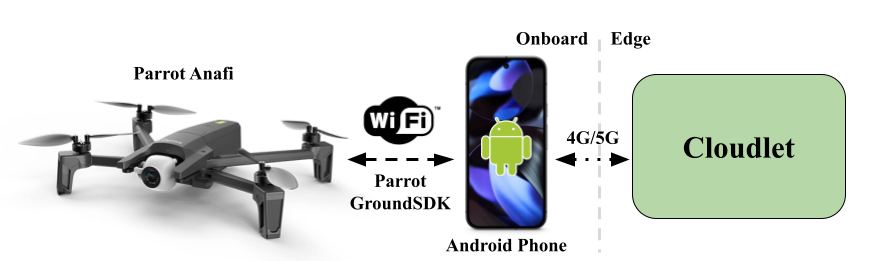
\includegraphics[width=1.0\linewidth]{chapter3/FIGS/onboard-phone.png}
    \caption{Android Phone Control~\cite{ParrotAnafi}}
    \label{fig:phone-control}
\end{figure}

Now that I had selected a device, it was time to mount it onboard the drone. For my initial mount, to save weight, I used industrial strength velcro and rubber bands. The drone was able to fly autonomously with the phone onboard and offload its video stream to the edge. However, I observed strange flight characteristics which caused several crashes. Upon further investigation, I determined that the phone was interfering with the magnetometer on the drone. This was causing the drone to lose track of its bearing mid-flight and veer off course.

To solve this magnetic interference, I added a layer of EMI  (electro-magnetic interference) shielding between the phone and the drone chassis. The shielding was made of Mu-metal, a nickel-iron ferromagnetic alloy used to absorb electro-magnetic radiation~\cite{Orasugh2023}. After testing, I determined that this mostly negated the observed interference. Unfortunately, it also added significantly to the payload weight, so much so that it exceeded the maximum takeoff mass (MTOM) of the aircraft. Once an aircraft's payload surpasses MTOM, it cannot fly because the lift it generates is no longer greater than its weight. Even with the lightest Android smartphones available, like the 61~g Unihertz Jelly Pro, the added weight of EMI shielding exceeded the Anafi's MTOM. 

As a result of the interference and MTOM restrictions, I was forced to abandon the phone prototype. It was too heavy for the Parrot Anafi hardware. I began searching for an alternative COTS device, much lighter than the Pixel 4a, but with the same broad specifications (self-contained, WiFi and cellular, self-powered, able to run Parrot GroundSDK or Olympe). 

\subsection{Smartwatch}
While mobile phones are the best SWaP-optimized devices on the market, smartwatches are by far the lightest, self-contained, commercially available computers. For many years, they were designed to operate in tandem with a phone, acting as a kind of always-visible secondary display. As time progressed, smartwatches grew more independent, incorporating more connectivity options and mounting more internal compute. The fitness community was a driving force behind this transformation. Many runners, for example, wanted a very small, lightweight, wearable device that could track their progress, contact emergency services, and play music on the move. In the late 2010s and early 2020s, this resulted in smartwatch products with cellular connectivity and enough local compute to run basic applications.

In many ways, smartwatches are the perfect device for SteelEagle's use case. They are extremely lightweight (less than 30~g compared to over 100~g for a phone), self-powered, cellular and WiFi-enabled, and able to run a slimmed-down Android (WearOS). For my smartwatch-based prototype, I chose the Samsung Galaxy Watch 4. At the time, this was the lightest cellular-capable Android smartwatch available. The Samsung Galaxy Watch 4 weighs just 25~g.

\begin{figure}
    \centering
    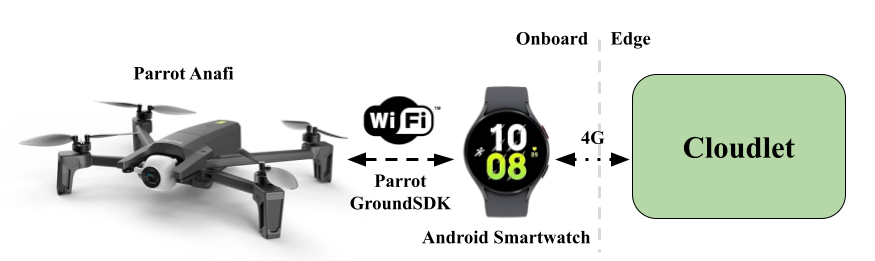
\includegraphics[width=1.0\linewidth]{chapter3/FIGS/onboard-watch.png}
    \caption{Android Watch Control~\cite{ParrotAnafi}}
    \label{fig:watch-control}
\end{figure}

After porting Parrot GroundSDK to WearOS, I was able to establish a 4G connection from the edge to the watch while autonomously piloting the drone via onboard software (Figure~\ref{fig:watch-control}). Now, all that was left to do was to physically mount the watch on the drone. I used a 3D-printed harness for this task, which clips onto the Parrot Anafi's removable battery. The harness weighs an additional 14~g, bringing the total payload weight to 39~g. Figure~\ref{fig:harness} shows the full assembly mounted on the aircraft. This brings the total take-off weight to 359~g, just 109~g above the 250~g FAA regulation threshold. Through rigorous testing, I determined that the watch payload did not exhibit the same negative flight characteristics as the Pixel 4a payload. It did not create as much EMI, likely because of its smaller size and lower power draw, and thus no shielding was needed. Additionally, the weight of the payload was far below the Anafi's MTOM, even with the added 3D printed mount to securely fasten it onboard.

The Samsung Galaxy Watch 4 finally yielded a successful prototype. The watch payload was able to autonomously fly the drone while maintaining a cellular connection to the edge. However, much work still remained unfinished. In particular, the drone's RTSP video stream would need to be transmitted to the edge in order to run the AI algorithms responsible for true autonomy: object detection, image segmentation, and obstacle avoidance among others. This would prove to be a formidable obstacle that pushed the watch hardware to its limit.

\begin{figure}
    \centering
    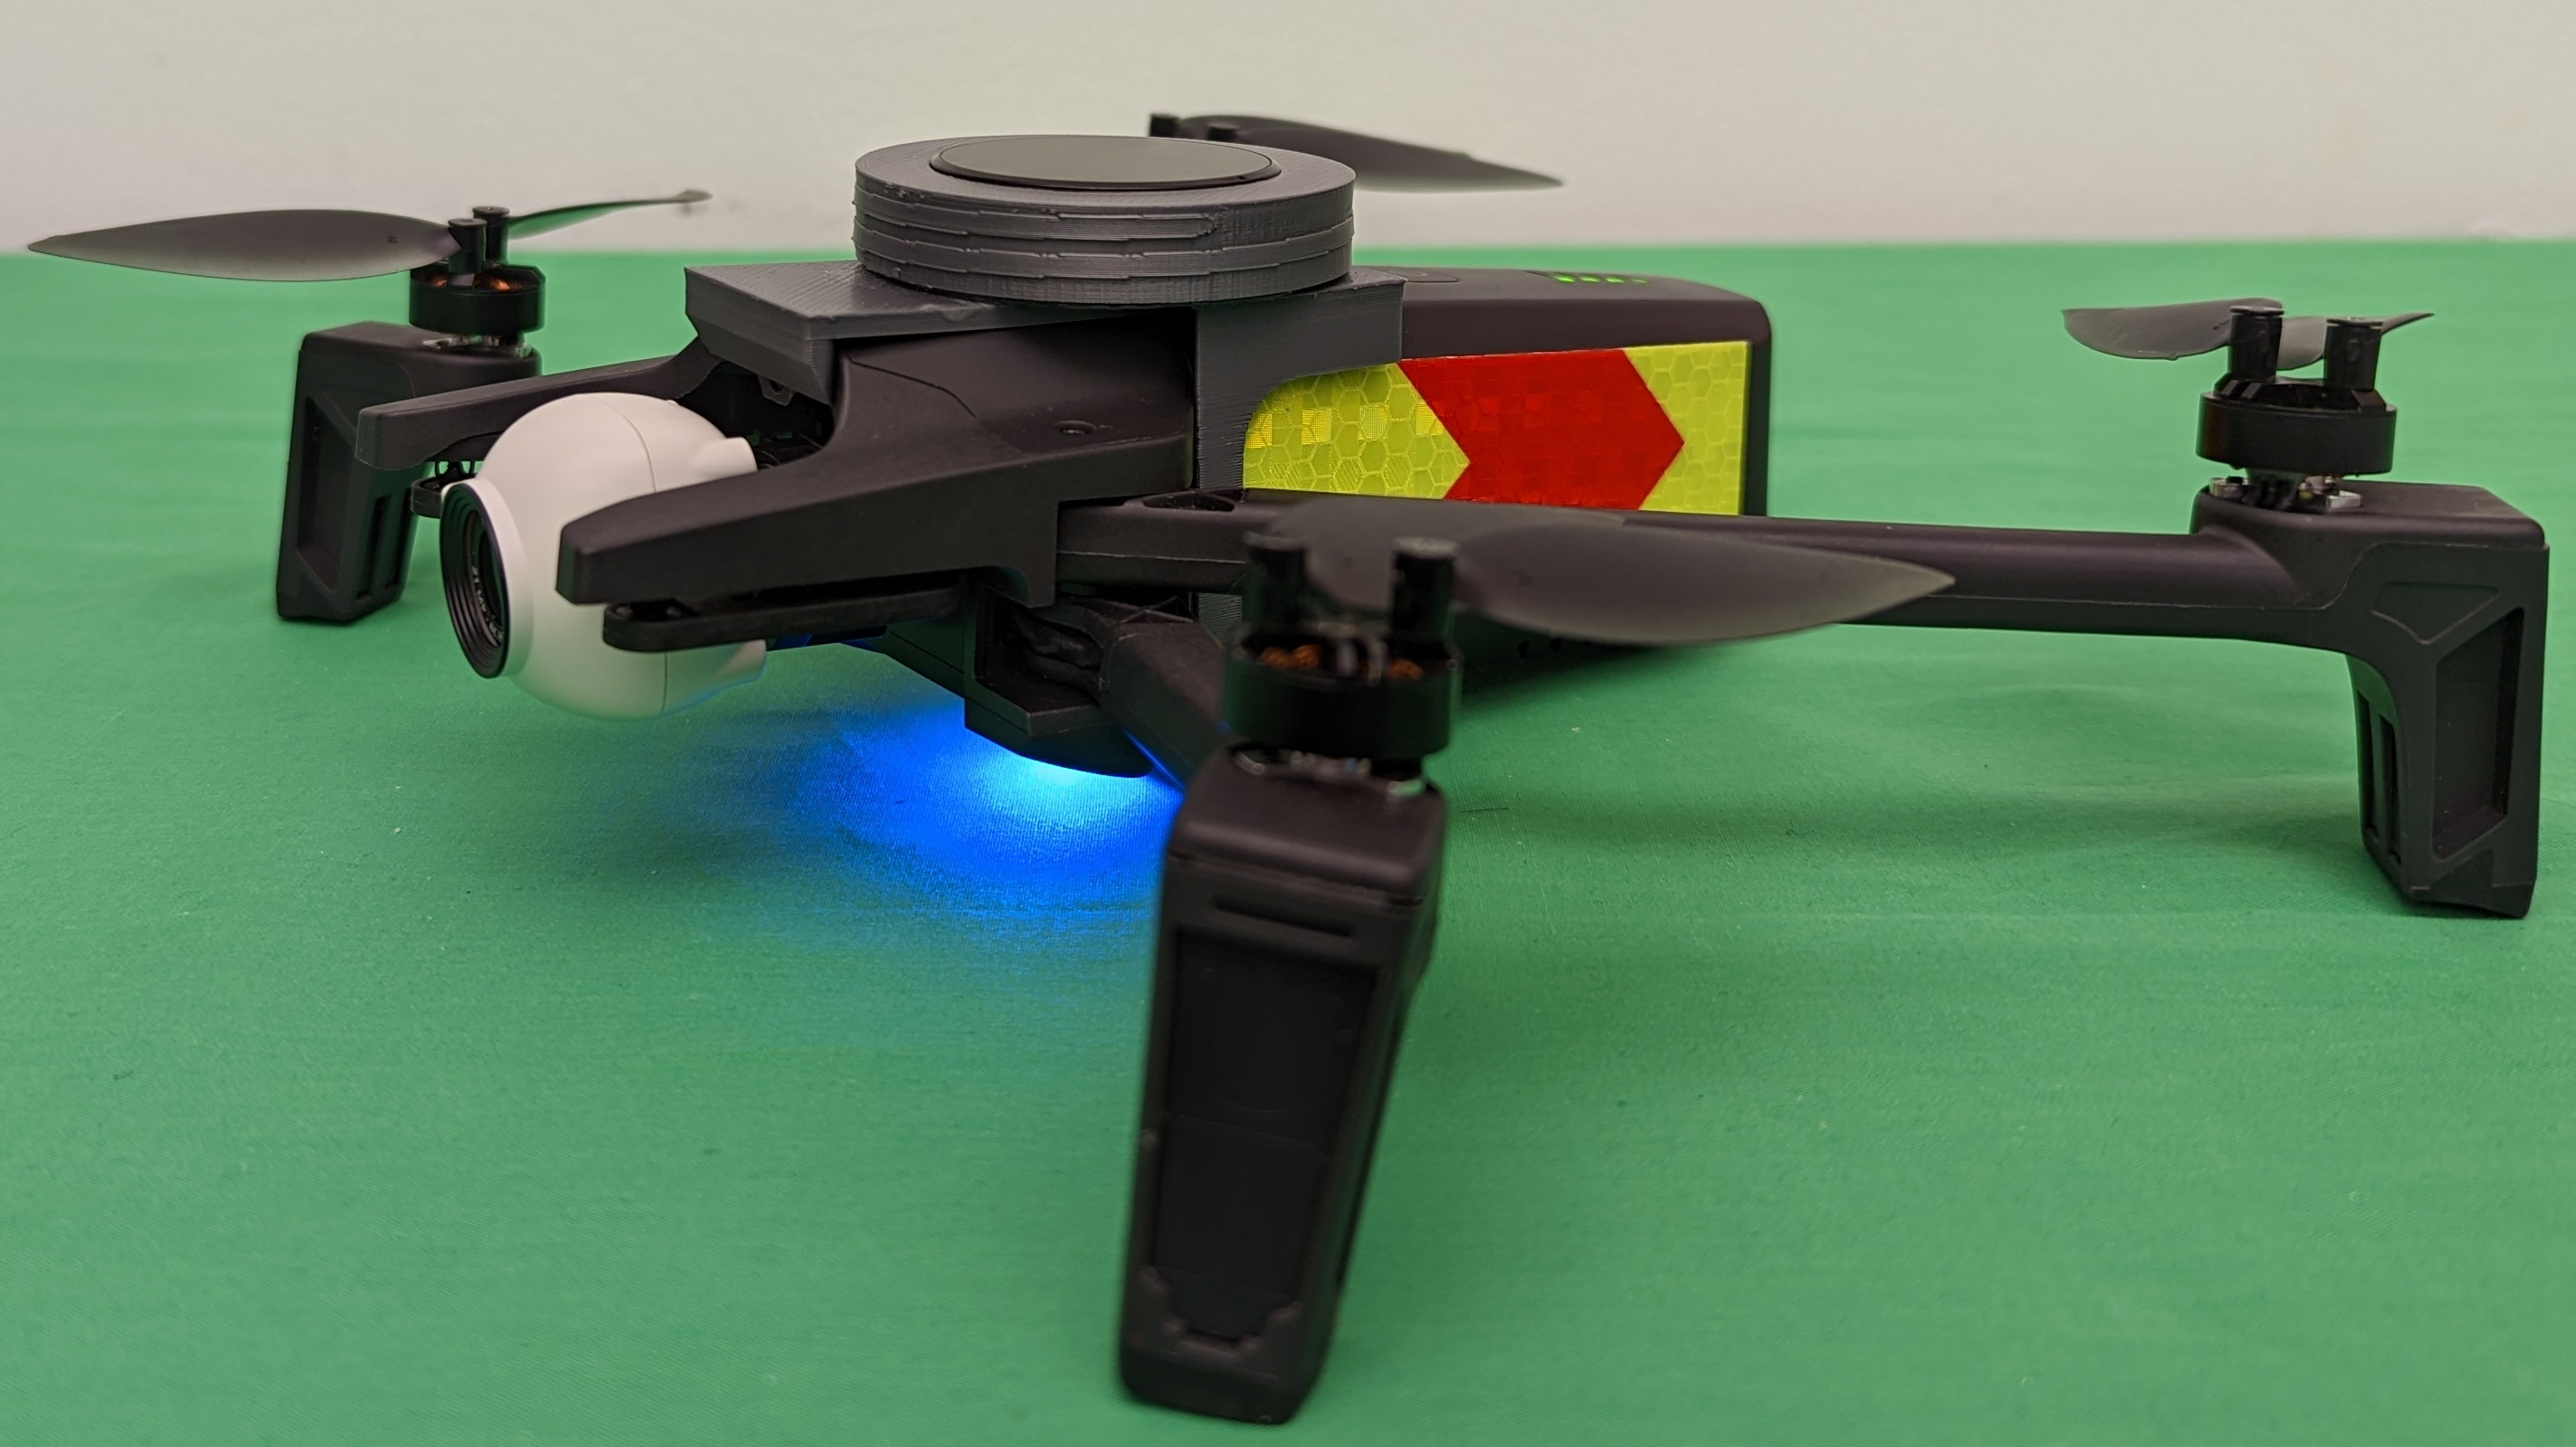
\includegraphics[width=0.6\linewidth]{chapter3/FIGS/drone-watch-combo.jpg}
    \caption{Drone with Watch-Harness Payload}
    \label{fig:harness}
\end{figure}

\section{An Austere Computing Environment}
\label{sec:austere-computing}
The watch is an austere computing environment with a dual-core
1.18~GHz ARM Cortex-A55 processor, 1.5 GB RAM, and 16 GB flash.
Table~\ref{tab:austerity} compares its attributes to the Google Pixel 4a and to the Unihertz Jelly Pro, the lightest-available Android smartphone. As wearable hardware, the watch has stringent thermal protection to shut itself down if its temperature approaches hardware limits. In addition, since wearables are meant to be worn, these hardware temperature limits must be much lower than traditional computers to prevent skin burns~\cite{Hepokoski2021}. Both computing and network transmission cause watch temperature to rise significantly.

This is a major problem, especially since in my design, the watch offloads the drone video stream to the edge. Typically, streaming tasks are both compute and transmission intensive. The act of sending frames too often or decoding frames onboard could cause overheating. In the case of the Samsung Galaxy Watch 4, overheating is detected by the operating system which in turn triggers a thermal shutdown. If this occurs, all currently running applications are suspended and the watch goes into hibernation until it is cool enough to proceed. A thermal shutdown in-flight would turn off the Parrot GroundSDK software running onboard and would thus trigger a pilot disconnection event on the drone. When this occurs, the drone returns automatically to its takeoff GPS location and lands. While this is far from disastrous, it would certainly be a serious handicap. As a result, the watch must be conservative in its network transmission and onboard computation in order to prevent overheating.

On the other hand, the agility and accuracy of the computer vision algorithms running at the edge are critically dependent on the attributes of the video stream. These algorithms determine the overall performance of the system; they are the ``brain'' that enables fully-autonomous operation. If the video stream delivered to them is hindered, performance will be directly affected. In order for this system to be effective, the watch must deliver as high fidelity a stream to the edge as possible without compromising its thermal limits. This is a delicate balancing act.

\begin{figure}
\centering
\begin{tabular}{|l|c|c|c|}
\hline
    & Samsung & Unihertz & Google \\
    & Galaxy & Jelly & Pixel\\
    & Watch 4 & Pro & 4a \\
\hline
Weight & 26~g & 61~g & 143~g\\
CPU cores & 2 & 4 & 8 \\
CPU speed & 1.18~GHz&1.45~GHz & 2.2~GHz\\
Memory & 1.5~GB & 3~GB & 6~GB\\
\hline
\end{tabular}
\caption{Austerity of Mobile Hardware}
\label{tab:austerity}
\end{figure}

\subsection{Anatomy of the Drone Video Stream}
\label{sec:anatomy-drone-stream}
The Parrot Anafi produces an encoded 720p 30fps video stream. It is produced on the drone's hardware and thus \textit{cannot be modified}. It is generated over the drone's WiFi network and can only be consumed by a single client on the network. Unlike most video streams, this stream uses an \textit{intra-refresh slice-decode} encoding scheme. An intra-refresh slice-decode encoding scheme is a streaming paradigm designed to minimize the visual impact of packet loss. 

To understand this special encoding scheme, first consider a normal H.264 video stream. The encoding scheme for these streams involves two types of data: complete frames (I frames) and inter frames (P and B frames). A complete frame is a full photo capture of a moment in time. When a complete frame is transmitted, it requires no additional data to decode. The trade-off is that complete frames are bandwidth hungry. An individual 720p complete frame can be several
KBs of data. By contrast, inter frames only capture the \textit{change from the previous frame}. They require reference data in order to decode, and are meaningless on their own. Their advantage is that they are very bandwidth efficient, sometimes on the order of a few hundred bytes in size. An H.264 video stream operates by transmitting a complete frame followed by a set amount of inter frames before looping back. This preserves fidelity by smoothing out gaps between complete frames with inter frames but also preserves bandwidth by sparingly transmitting complete frames.

There is one major negative of typical H.264 video streams in the context of mobile devices: they are not resilient to packet loss. On the Internet, which is a mostly wired network, this is not a serious problem. But, over the air, packet loss is frequent. If a complete frame is lost, this kind of stream must shut down until a new one can be broadcast; all following inter frames will have no complete frame to refer to and will be rendered useless. Usually this can take a whole second or more, during which a drone pilot, for example, would not be able to see.

An intra-refresh slice-decode scheme takes a different approach. Instead of complete frames and inter frames, this scheme splits a single frame into \textit{slices}. These slices capture a sliver of data horizontally across a frame. When a frame is transmitted, the encoder allocates one slice to be the ``complete slice'' (I slice) and the rest to be ``inter slices'' (P slices). Figure~\ref{fig:slice-encoding} shows a breakdown of how each set of frames transmitted by the Anafi are organized. Each inter slice is only dependent upon its section of the frame; they are completely independent of each other. 

This has two positive attributes. The first is that this minimizes the impact of packet loss on a single frame. If a single frame is dropped, only one slice of the frame loses its complete slice reference. In this case, that section of the frame is corrupted until a new complete slice is sent. Otherwise, the rest of the frame is decoded normally. The second benefit of this approach is that it keeps bandwidth usage consistent. With a traditional stream, bandwidth usage spikes when complete frames are sent but then plummets when inter frames are sent. In this scheme, since every frame has approximately the same size (one complete slice with the rest being inter slices), bandwidth usage stays somewhat constant. This is useful because other applications can now plan around its tight usage bound.

\begin{figure}
    \centering
    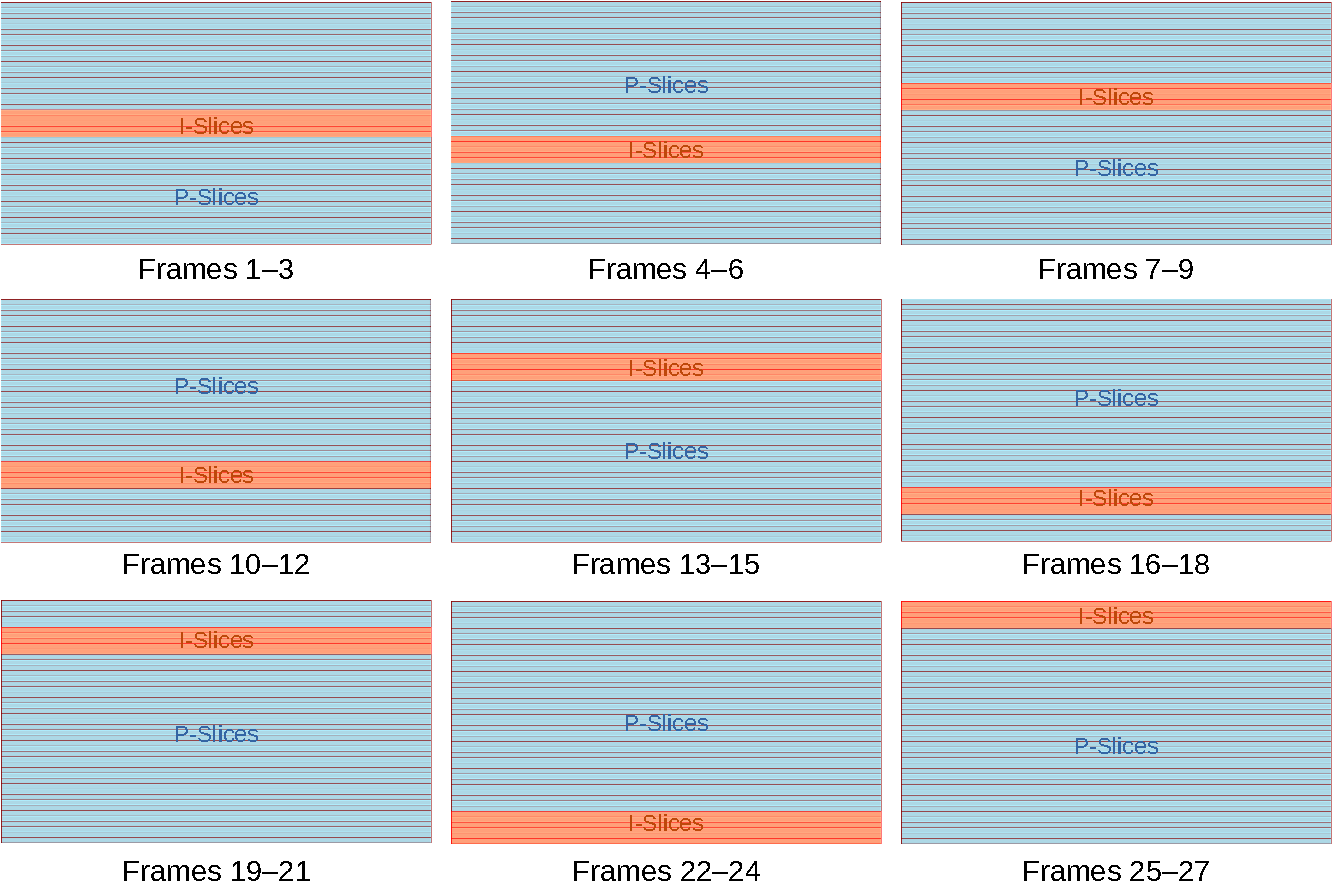
\includegraphics[width=0.9\linewidth]{chapter3/FIGS/slice-encoding-crop.pdf}
    \begin{captext}
    \\[0.1cm] \small Each segment of three frames contains one I-slice (shown in orange) and transmits the remaining slices as P-slices (shown in blue). The I-slice that is sent is chosen from the center of the frame going outward. After 30 frames, the process starts from the beginning.
    \end{captext}
    \caption{Intra-Refresh Slice-Decode Stream}
    \label{fig:slice-encoding}
\end{figure}

\subsection{The Video Stream on the Watch}
There are two obvious methods for offloading the drone video stream from the watch to the edge. The first is to decode the drone stream on the watch and then ship the decoded frames to the edge. This allows the watch to throttle its send rate to account for 4G transmission overheating. The second is to directly offload the stream packets from the drone network to the cloudlet, where they can then be decoded. This involves the least amount of computation power on the watch, but requires a higher transmission rate. I will refer to these as method 1 and method 2 respectively.

\subsubsection{Method 1: Decode-on-Device}
\label{sec:method-1}
Decode-on-device involves the watch decoding the drone video stream then sending decoded frames individually to the edge. This allows for some pre-processing on the watch side, such as downscaling or stream throttling for bandwidth saving. Unfortunately, the Anafi's intra-refresh slice-decode stream poses a major hurdle to this method's success: due to its construction, \textit{every frame must be decoded in order to maintain a coherent stream}. This is in stark contrast to a typical stream, which only requires the I frames (usually generated at around 1~fps) to be decoded to maintain coherence. As such, any device consuming the drone stream must decode one frame every 33~ms on average to keep up with the 30~fps output and prevent drifting latency, regardless of cellular transmission throughput. Drifting latency is a phenomenon where latency increases over time due to queueing delay. If a device drops packets to keep up with this strict time bound, it could cause some loss of quality as important I slices are discarded. On most devices, this is not an issue. But on the constrained compute of the Galaxy Watch 4, even relatively light workloads are considered difficult. Table~\ref{tab:decoding-time} shows the time taken to decode a frame of the Anafi's video stream by the watch, the Pixel 4a, and the Unihertz Jelly Pro. As shown, both the watch and the Jelly Pro cannot decode fast enough to maintain stable latency.

\begin{table}
        \centering
        \begin{tabular}{|l|c|}
                \hline
                & Decode Time \\
                \hline
                Samsung Galaxy Watch & \color{red}{55ms} \\
                Unihertz Jelly Pro & \color{red}{35ms} \\
                Google Pixel 4a & 25ms \\
                \hline
        \end{tabular}
        \begin{captext}
                \centering
                \\[0.1cm] \small \color{red}Red denotes a decode rate that is  too slow at 30~FPS.
        \end{captext}
        \caption{Average Decoding Time by Platform}
        \label{tab:decoding-time}
\end{table}

\begin{table}
\centering
\begin{tabular}{|r|c|c|}
\hline
Sleep&\multicolumn{2}{|c|}{Payload Size}\\
\cline{2-3}
Interval & 35~KB& 100~KB\\
\hline
33 ms & \redcross & \redcross \\
100 ms & \redcross & \redcross \\
500 ms & \redcross & \redcross \\
800 ms & \redcross & \redcross \\
1000 ms & \greencheck & \greencheck \\
\hline
\end{tabular}
\begin{captext}
\\[0.1cm]
\redcross\hspace{0.1in} thermal shutdown\\
\greencheck\hspace{0.1in} no thermal shutdown
\end{captext}
\caption{Effect of Sleeps}
\label{tab:thermal-sensitivity}
\end{table}

\subsubsection{Method 2: Pass-Through Streaming}
\label{sec:method-2}
An easy way to avoid decoding on device is to directly send the drone stream packets over cellular to the cloudlet, where they can then be decoded. With this method, computation on the device is minimal but network transmission is much more frequent. This is a good tradeoff in many cases, but on the watch, heavy transmission workloads may cause overheating. To determine the effect of transmission on the watch thermals, I devised a simple experiment: the watch sends a variable size packet, representing typical stream packet sizes (35KB up to 100KB), over the network with variable sleep times in between sends. There is no video stream or other onboard computation involved, only raw transmission. Table~\ref{tab:thermal-sensitivity} shows the results of this experiment. It is clear that the bottleneck on the watch is not the packet size but the send rate. Any send rate above 1~Hz causes thermal shutdown. This means that pass-through streaming is mostly out of the question.

\begin{figure}
    \centering
    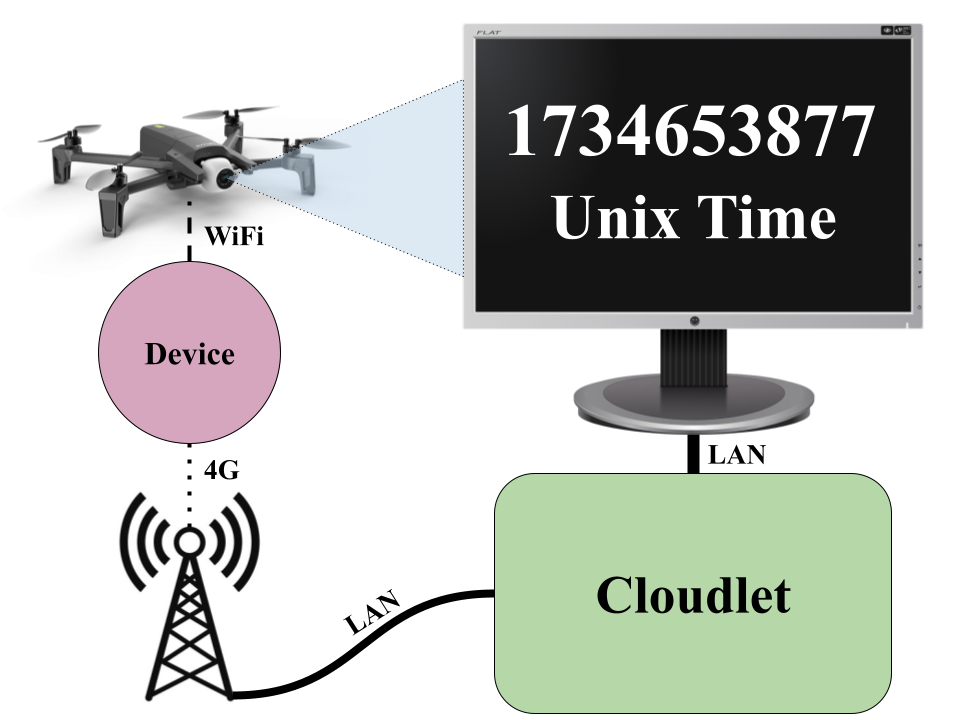
\includegraphics[width=0.75\linewidth]{chapter3/FIGS/mtp-experiment.png}
    \begin{captext}
    \\ \small The drone camera captures UNIX time displayed on a monitor that is connected to the cloudlet. It then sends the video stream over the device to the cloudlet. The total latency is the difference between the observed time in the stream versus the actual time the frame was received.
    \end{captext}
    \caption{Streaming Experiment}
    \label{fig:streaming-experiment}
\end{figure}

\section{The Quest for a Working Stream}
\label{sec:quest-working-stream}
A successful stream to the cloudlet must have acceptable latency, throughput, and image quality. Without these aspects, the stream will not be usable by AI algorithms running on the edge and therefore cannot contribute to fully-autonomous operation. Specifically, the stream must have:
\begin{itemize}
    \item \textbf{Sustainability}: the watch stream must sustain itself for the duration of a drone flight (at least 20 minutes).
    \item \textbf{Stable Latency}: the watch stream must process frames on average equal to or faster than 33~ms to keep up with the 30~fps stream from the drone.
    \item \textbf{High-Quality Frames}: the watch stream must deliver ``quality'' images to the cloudlet that lack significant visual artifacts and can thus be used by computer vision algorithms.
\end{itemize}
The austere environment on the watch makes achieving such a stream a challenge. The watch cannot decode frames fast enough to maintain stable latency, and thus cannot decode-on-device and send at a throttled framerate. It also cannot transmit consistently enough to pass-through stream from the drone to the cloudlet without decoding. To discover a path forward, I devised a set of experiments that would better characterize the bottlenecks in the system. By understanding these bottlenecks, an effective solution could be found.

\subsection{Experimental Setup}
\label{sec:streaming-experiment-setup}
For each of the following experiments, the setup is identical. The drone is started so that its RTSP stream and WiFi network are initialized. Then, the client device is connected to the drone’s WiFi network and the stream application is launched on the device. The application uses a variable method to stream image data from the drone to a cloudlet. When the frame arrives at the cloudlet, it is saved along with its time of arrival. The drone’s camera is pointed at a screen connected directly to the cloudlet which is displaying the current UNIX timestamp. By comparing the UNIX timestamp in the received image and its time of arrival, the transmission latency can be determined in post processing. The UNIX timestamp can also be used to determine the time at which thermal shutdown occurs. Figure~\ref{fig:streaming-experiment} shows the experimental setup. For experiment 1 and 2, I provide two other devices, the Google Pixel 4a and the Unihertz Jelly Pro as baselines. The duration of the experiments in all cases is the duration of a drone flight: 20 minutes.

\begin{table}
\centering
\begin{tabular}{|l|c|c|c|c|}
\hline
    & Pass- & Decode & Decode & Decode \\
    & Through & No & 3~fps & 1~fps \\
    & Stream & Throttle & Throttle & Throttle \\
\hline
Samsung Galaxy Watch 4 & \cellcolor{red!20}68~s & \cellcolor{red!20}380~s & \cellcolor{red!20}565~s & \cellcolor{green!20}DNO \\[0.1cm]
\hline
Unihertz Jelly Pro & \cellcolor{green!20}DNO & \cellcolor{red!20}TT & \cellcolor{red!20}TT & \cellcolor{green!20}DNO  \\[0.1cm]
\hline
Google Pixel 4a & \cellcolor{green!20}DNO & \cellcolor{green!20}DNO & \cellcolor{green!20}DNO & \cellcolor{green!20}DNO \\[0.1cm]
\hline
\end{tabular}
    \begin{captext}
    \\[0.1cm] \small Time in seconds before the device experiences a thermal shutdown. DNO means that the device did not overheat for the duration of the experiment (20~minutes). TT means that the device experienced thermal-related CPU throttling which affected performance.
    \end{captext}
\caption{Experiment 1: Sustainability}
\label{tab:time-before-overheating}
\end{table}

\subsection{Experiment 1: Sustainability}
\label{sec:exp1-sustainability}
In this experiment, I timed each device running either decode-on-device (Method 1~\S\ref{sec:method-1}) or pass-through (Method 2~\S\ref{sec:method-2}). For the decode-on-device runs, I added additional tests with throttling. In these cases, the device decodes at the full frame rate but only sends to the cloudlet at the specified framerate. Table~\ref{tab:time-before-overheating} shows the results of the experiment. The watch clearly cannot sustain pass-through streaming for any significant duration (about 1 minute), and can sustain non-throttled and 3~fps throttled streaming for up to 9 minutes.  However, the 1~fps throttled stream did not overheat for the duration of the test. This implicates 4G transmission as the main thermal bottleneck and sets an upper-bound for transmission frequency at 1~Hz. The Google Pixel 4a, unsurprisingly, breezed through all four tests. The Jelly Pro had trouble with the higher send rate of some decode-on-device tests but was overall good. This shows that slightly better thermals would drastically improve sustainable performance on the watch. 


\subsection{Experiment 2: Stable Latency}
In this experiment, I setup each device running the same methods as in Section~\ref{sec:exp1-sustainability}. This time, I measured the stream latency over the course of the test. Table~\ref{tab:stable-latency} shows the results of the experiment. No method provided a stream with stable latency on the watch. On the Jelly Pro, only the 1~fps throttled stream did. This implies that for the non-throttled and 3~fps throttled stream, the network transmission affected the decoding performance, slowing it down and causing latency to drift. On the Pixel 4a, all decode-on-device methods provided stable latency. No device successfully performed pass-through streaming without drift. Clearly, a different approach is needed on the watch to guarantee consistent latency.

\begin{table}
\centering
\begin{tabular}{|l|c|c|c|c|}
\hline
    & Pass- & Decode & Decode & Decode \\
    & Through & No & 3~fps & 1~fps \\
    & Stream & Throttle & Throttle & Throttle \\
\hline
Samsung Galaxy Watch 4 & \cellcolor{red!20}DRIFT & \cellcolor{red!20}DRIFT & \cellcolor{red!20}DRIFT & \cellcolor{red!20}DRIFT \\[0.1cm]
\hline
Unihertz Jelly Pro & \cellcolor{red!20}DRIFT & \cellcolor{red!20}DRIFT & \cellcolor{red!20}DRIFT & \cellcolor{green!20}1~s  \\[0.1cm]
\hline
Google Pixel 4a & \cellcolor{red!20}DRIFT & \cellcolor{green!20}1~s & \cellcolor{green!20}1~s & \cellcolor{green!20}1~s \\[0.1cm]
\hline
\end{tabular}
    \begin{captext}
    \\[0.1cm] \small Latency in seconds. DRIFT means that the latency drifted over the duration of the experiment (20~minutes).
    \end{captext}
\caption{Experiment 2: Stable Latency}
\label{tab:stable-latency}
\end{table}

\begin{table}
\centering
\begin{tabular}{|l|c|c|c|c|}
        \hline
        & $c = 1$ & $c = 2$ & $c = 3$ & $c = 4$ \\[0.1cm]
        \hline
$d = 1$ & 7~s, 80\% & 7~s, 80\%	& 8s, 90\%	& 8~s, 70\% \\[0.1cm]
\hline
$d = 2$ & 7~s, 80\% & 7~s, 80\% & 7~s, 90\%	& 7~s, 80\% \\[0.1cm]
\hline
$d = 3$ & 1~s, 30\% & \cellcolor{green!20}1~s, 99\%	& 4~s, 60\% & 4~s, 50\% \\[0.1cm]
\hline
$d = 4$ & $\leq$ 5\% & 1~s, 50\% &	1~s, 10\% & 6~s, 30\% \\[0.1cm]
\hline
\end{tabular}
    \begin{captext}
    \\[0.1cm] \small Latency in seconds followed by the approximate percentage of visual-artifact-free frames produced during the test. Combinations off the grid did not produce acceptable results, either due to drifting latency or poor quality. Visual quality is determined subjectively.
    \end{captext}
\caption{Experiment 3: High-Quality Frames}
\label{tab:hq-frames}
\end{table}

\subsection{Experiment 3: High-Quality Frames}
If the watch decodes the stream as outlined in Method 1~\S\ref{sec:method-1}, it produces very high-quality images with no visual artifacts at the cost of drifting latency. This is not acceptable by the standards outlined earlier in Section~\ref{sec:quest-working-stream}. Even so, room for compromise remains. While not desirable, intentional packet dropping of the video stream prior to decoding is an effective way to reduce latency at the cost of quality, since fewer stream packets reduces the time spent decoding. In this experiment, I determine how much packet dropping is acceptable to preserve quality. I test the watch under the 1~fps throttled decode-on-device workload, decoding chunks of $c$ packets and then subsequently dropping $d$ packets. For example, a $c=2, d=2$ scheme would involve decoding 2 out of every 4 packets. Table~\ref{tab:hq-frames} shows the results of the experiment. As $d$ increases, quality drops but latency decreases as the average time to decode shrinks. In the other direction, as $c$ increases, latency generally increases too since the average time to decode grows. At $c=2, d=3$, there is a sweet-spot where the watch latency is minimal and the impact on frame quality is also minimal. It is this combination that finally produces a workable stream.

\begin{figure}
    \centering
    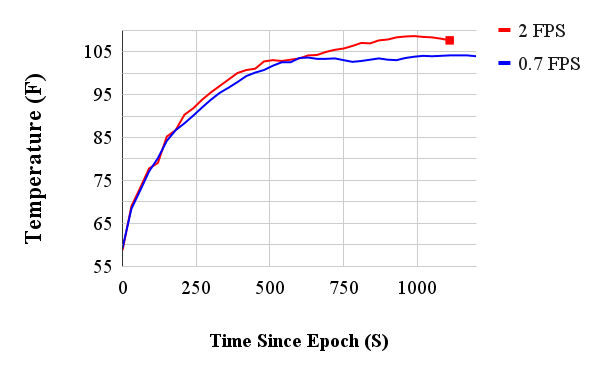
\includegraphics[width=0.8\linewidth]{chapter3/FIGS/temperature.png}
    \begin{captext}
    \\[0.1cm]
    \small The red square at the end of the 2~fps temperature curve indicates a thermal shutdown occurred. The 0.7~fps graph continues without overheating.
    \end{captext}
    \caption{Watch Temperature at Different Throttling Levels}
    \label{fig:temperature}
\end{figure}

\subsection{The Stream in Practice}
\label{sec:stream-in-practice}
Putting together the results of the three experiments, a working solution emerges. It solves each of the requirements presented in Section~\ref{sec:quest-working-stream}:
\begin{itemize}
    \item \textbf{Sustainability}: \textit{the watch stream must sustain itself for the duration of a drone flight (at least 20 minutes).}
    The watch throttles sending frames to the cloudlet to 1~Hz which is sustainable for 20 minutes.
    \item \textbf{Stable Latency}: \textit{the watch stream must process frames on average equal to or faster than 33~ms to keep up with the 30~fps stream from the drone.}
    The watch drops 3 packets for every 2 it decodes which reduces the average decode time enough to keep up with the drone stream.
    \item \textbf{High-Quality Frames}: \textit{the watch stream must deliver ``quality'' images to the cloudlet that lack significant visual artifacts and can thus be used by computer vision algorithms.}
    The watch decodes enough packets to maintain a high-quality stream.
\end{itemize}
Integrated into the larger application, parts of this streaming scheme must be modified to make way for other compute resources. In particular, throttling to 1~fps proves too demanding once other processes are factored in. Once throttling is dropped to 0.7~fps, the stream once again is functional. Figure~\ref{fig:temperature} shows the watch temperature over time with a 2~fps and a 0.7~fps throttled stream within the larger application. At 2~fps, the stream experiences thermal shutdown once the watch reaches an external temperature of 108\degree F. At 0.7~fps, the watch maintains an external temperature under 105\degree F for 20 minutes without ever experiencing a thermal shutdown.

With the stream now working, the Parrot Anafi has successfully been connected to the edge via its Galaxy Watch 4 payload. The watch can offload the drone's video stream over 4G at 0.7~fps with 1~s latency while simultaneously sending actuation commands. The drone can also operate BVLOS without the need for any connected human pilots. Now, all that is needed is a complementary edge software backend that can provide the drone with the intelligence required for full autonomy.

